\documentclass{uofa-eng-assignment}
\usepackage{amsmath}
\usepackage{enumerate}% http://ctan.org/pkg/enumerate
\usepackage{lipsum}
\usepackage{hyperref}
\usepackage{amsmath, amsthm, amssymb, amsfonts, physics}
\usepackage{mathtools}
\usepackage{graphicx}
\usepackage{fdsymbol}

\hypersetup{
    colorlinks=true,
    linkcolor=blue,
    filecolor=magenta,
    urlcolor=cyan,
    pdftitle={Overleaf Example},
    pdfpagemode=FullScreen,
}

\graphicspath{ {./images/} }

\DeclareRobustCommand{\rchi}{{\mathpalette\irchi\relax}}
\newcommand{\infdiv}{D\infdivx}
\newcommand{\irchi}[2]{\raisebox{\depth}{$#1\chi$}} % inner command, used by \rchi
\newcommand\aug{\fboxsep=-\fboxrule\!\!\!\fbox{\strut}\!\!\!}
\newcommand*{\name}{\textbf{Luke Nguyen}}
\newcommand*{\id}{\textbf{D5850A}}
\newcommand*{\course}{Statistical Methods and Data Analysis (EN.625.603)}
\newcommand*{\assignment}{Problem Set 6}

\begin{document} \maketitle
%%%%%%%%%%%%%%%%%%%%%%%%%%%%%%%%%%%%%%%%%%%%%%%%%%%%%%%%%%%%%%%%%%%%%%%%%%%%%%%%%%%%%%%%%%%%%%%%%%%%    
\begin{enumerate}
    %%%%%%%%%%%%%%%%%%%%%%%%%%%%%%%%%%%%%%%%%%%%%%%%%%%%%%%%%%%%%%%%%%%%%%%%%%%%%%%%%%%%%%%%%%%%%%%%%%%%    
    %%%%%%%%%%%%%%%%%%%%%%%%%%%%%%%%%%%%%%%%%%%%%%%%%%%%%%%%%%%%%%%%%%%%%%%%%%%%%%%%%%%%%%%%%%%%%%%%%%%%    
    %%%%%%%%%%%%%%%%%%%%%%%%%%%%%%%%%%%%%%%%%%%%%%%%%%%%%%%%%%%%%%%%%%%%%%%%%%%%%%%%%%%%%%%%%%%%%%%%%%%%    
    %%%%%%%%%%%%%%%%%%%%%%%%%%%%%%%%%%%%%%%%%%%%%%%%%%%%%%%%%%%%%%%%%%%%%%%%%%%%%%%%%%%%%%%%%%%%%%%%%%%%    
    %%%%%%%%%%%%%%%%%%%%%%%%%%%%%%%%%%%%%%%%%%%%%%%%%%%%%%%%%%%%%%%%%%%%%%%%%%%%%%%%%%%%%%%%%%%%%%%%%%%%    
    \item[]
        \textbf{Question 6.2.8b} \\
        Calculate the $P-$values for the hypothesis tests indicated in Question 6.2.1. \\
        Do they agree with your decision on whether or not to reject $H_0$? \\
        \textbf{(b)}
        ${H_0\!:\mu} = 42.9$ versus $H_1\!:\mu \neq 42.9; \bar{y} =45.1, n=16, \sigma = 3.2, \alpha = 0.01$. \\
        \textbf{Solution} \\
        Applying \textbf{Theorem 6.2.1(c)}, the test at the $\alpha$ level of significance
        \begin{align*}
            \text{Reject}\;H_0\;\text{if}\;|z| > z_{\alpha/2} = z_{0.005} = 2.575 \\
            \text{where}\;z = \frac{\bar{y} - \mu_0}{\sigma / \sqrt{n}} = \frac{45.1 - 42.9}{3.2 / \sqrt{16}} = 2.75
        \end{align*}
        Therefore, we reject $H_0$; \\
        Using \textbf{Definition 6.2.4}, we calculate $P$-value as follows
        \begin{align*}
            P\text{-value} = 2 \times P(z > 2.75) = 2 \times (1 - P(z < 2.75)) = 2 \times (1 - 0.997) = \boldsymbol{0.006}
        \end{align*}
        Since $P\text{-value} < \alpha$, we reject $H_0$ and \textbf{it agrees with the decision on rejecting $\boldsymbol{H_0}$}.
        %%%%%%%%%%%%%%%%%%%%%%%%%%%%%%%%%%%%%%%%%%%%%%%%%%%%%%%%%%%%%%%%%%%%%%%%%%%%%%%%%%%%%%%%%%%%%%%%%%%%    
        %%%%%%%%%%%%%%%%%%%%%%%%%%%%%%%%%%%%%%%%%%%%%%%%%%%%%%%%%%%%%%%%%%%%%%%%%%%%%%%%%%%%%%%%%%%%%%%%%%%%    
        %%%%%%%%%%%%%%%%%%%%%%%%%%%%%%%%%%%%%%%%%%%%%%%%%%%%%%%%%%%%%%%%%%%%%%%%%%%%%%%%%%%%%%%%%%%%%%%%%%%%    
        %%%%%%%%%%%%%%%%%%%%%%%%%%%%%%%%%%%%%%%%%%%%%%%%%%%%%%%%%%%%%%%%%%%%%%%%%%%%%%%%%%%%%%%%%%%%%%%%%%%%    
        %%%%%%%%%%%%%%%%%%%%%%%%%%%%%%%%%%%%%%%%%%%%%%%%%%%%%%%%%%%%%%%%%%%%%%%%%%%%%%%%%%%%%%%%%%%%%%%%%%%%    
    \item[]
        \textbf{Question 6.3.7} \\
        What $\alpha$ levels are possible with a decision rule of the form
        ``Reject $H_0$ if $k \geq k^*$'' when $H_0:p=0.5$ is to be tested against
        $H_1:p > 0.5$ using a random sample of size $n = 7$? \\
        \textbf{Solution} \\
        For a test of size $n = 7$, $p > 0.5$ we have the following scenarios
        \begin{itemize}
            \item $k = 4$
                  \begin{align*}
                      \alpha & = P(\text{Reject}\;H_0\;|\;H_0\;\text{is true})       \\
                             & = P(k \geq 4\;|\;p= 0.5)                              \\
                             & = \sum_{k=4}^{7} \binom{7}{k} (0.5)^k (1 - 0.5)^{7-k} \\
                             & = 0.5
                  \end{align*}
            \item $k = 5$
                  \begin{align*}
                      \alpha & = P(\text{Reject}\;H_0\;|\;H_0\;\text{is true})       \\
                             & = P(k \geq 5\;|\;p= 0.5)                              \\
                             & = \sum_{k=5}^{7} \binom{7}{k} (0.5)^k (1 - 0.5)^{7-k} \\
                             & = 0.2265625
                  \end{align*}
            \item $k = 6$
                  \begin{align*}
                      \alpha & = P(\text{Reject}\;H_0\;|\;H_0\;\text{is true})       \\
                             & = P(k \geq 6\;|\;p= 0.5)                              \\
                             & = \sum_{k=6}^{7} \binom{7}{k} (0.5)^k (1 - 0.5)^{7-k} \\
                             & = 0.0625
                  \end{align*}
            \item $k = 7$
                  \begin{align*}
                      \alpha & = P(\text{Reject}\;H_0\;|\;H_0\;\text{is true})       \\
                             & = P(k \geq 7\;|\;p= 0.5)                              \\
                             & = \sum_{k=7}^{7} \binom{7}{k} (0.5)^k (1 - 0.5)^{7-k} \\
                             & = 0.0078125
                  \end{align*}
        \end{itemize}
        Thus, the possible $\alpha$ levels are $\boldsymbol{0.5, 0.2265625, 0.0625, 0.0078125}$.
        %%%%%%%%%%%%%%%%%%%%%%%%%%%%%%%%%%%%%%%%%%%%%%%%%%%%%%%%%%%%%%%%%%%%%%%%%%%%%%%%%%%%%%%%%%%%%%%%%%%%    
        %%%%%%%%%%%%%%%%%%%%%%%%%%%%%%%%%%%%%%%%%%%%%%%%%%%%%%%%%%%%%%%%%%%%%%%%%%%%%%%%%%%%%%%%%%%%%%%%%%%%    
        %%%%%%%%%%%%%%%%%%%%%%%%%%%%%%%%%%%%%%%%%%%%%%%%%%%%%%%%%%%%%%%%%%%%%%%%%%%%%%%%%%%%%%%%%%%%%%%%%%%%    
        %%%%%%%%%%%%%%%%%%%%%%%%%%%%%%%%%%%%%%%%%%%%%%%%%%%%%%%%%%%%%%%%%%%%%%%%%%%%%%%%%%%%%%%%%%%%%%%%%%%%    
        %%%%%%%%%%%%%%%%%%%%%%%%%%%%%%%%%%%%%%%%%%%%%%%%%%%%%%%%%%%%%%%%%%%%%%%%%%%%%%%%%%%%%%%%%%%%%%%%%%%%    
    \item[]
        \textbf{Question 6.4.3} \\
        For the decision rule found in Question 6.2.2 to test $H_0\!:\mu = 95$ versus $H_1\!:\mu \neq 95$,
        at what $\alpha = 0.06$ level of significance, calculate $1 - \beta$ when $\mu = 90$. \\
        \textbf{Solution} \\
        From 6.2.2, we have $n = 22, \sigma = 15$, the decision rule for two-tailed is
        \begin{align*}
            \text{Reject}\;H_0\;\text{if}\;|z| > z_{\alpha/2} = z_{0.03} = 1.88                               \\
            \text{where}\;z = \frac{\bar{y} - \mu_0}{\sigma / \sqrt{n}} = \frac{\bar{y} - 95}{15 / \sqrt{22}} \\
            \absolutevalue{\bar{y} } > 1.88 \times \frac{15}{\sqrt{22}} + 95                                  \\
            \bar{y} > 101.01\;\text{or}\;\bar{y} < 88.99
        \end{align*}
        From \textbf{6.4}, we knnow that $1 - \beta = P(\text{Reject}\;H_0\;|\;H_1\;\text{is true})$, thus, we can
        calculate $1 - \beta$ as follows
        \begin{align*}
            1 - \beta & = P(\text{Reject}\;H_0\;|\;H_1\;\text{is true})                                       \\
                      & = P(\bar{y} > 101.01\;|\;\mu = 90) + P(\bar{y} < 88.99\;|\;\mu = 90)                  \\
                      & = P(z > \frac{101.01 - 90}{15 / \sqrt{22}}) + P(z <\frac{88.99 - 90}{15 / \sqrt{22}}) \\
                      & = P(z > 3.443) +  P(z < -0.317)                                                       \\
                      & = 0.0003 + 0.3765                                                                     \\
                      & = \boldsymbol{0.3768}
        \end{align*}
        %%%%%%%%%%%%%%%%%%%%%%%%%%%%%%%%%%%%%%%%%%%%%%%%%%%%%%%%%%%%%%%%%%%%%%%%%%%%%%%%%%%%%%%%%%%%%%%%%%%%    
        %%%%%%%%%%%%%%%%%%%%%%%%%%%%%%%%%%%%%%%%%%%%%%%%%%%%%%%%%%%%%%%%%%%%%%%%%%%%%%%%%%%%%%%%%%%%%%%%%%%%    
        %%%%%%%%%%%%%%%%%%%%%%%%%%%%%%%%%%%%%%%%%%%%%%%%%%%%%%%%%%%%%%%%%%%%%%%%%%%%%%%%%%%%%%%%%%%%%%%%%%%%    
        %%%%%%%%%%%%%%%%%%%%%%%%%%%%%%%%%%%%%%%%%%%%%%%%%%%%%%%%%%%%%%%%%%%%%%%%%%%%%%%%%%%%%%%%%%%%%%%%%%%%    
        %%%%%%%%%%%%%%%%%%%%%%%%%%%%%%%%%%%%%%%%%%%%%%%%%%%%%%%%%%%%%%%%%%%%%%%%%%%%%%%%%%%%%%%%%%%%%%%%%%%%    
    \item[]
        \textbf{Question 6.4.4} \\
        Construct a power curve for the $\alpha = 0.05$ test of $H_0\!:\mu = 60$ versus $H_1\!:\mu \neq 60$
        if the data consist of a random sample of size 16 from a normal distribution having $\sigma = 4$. \\
        \newpage
        \textbf{Solution} \\
        From \textbf{6.4}, \textit{a graph of $1 - \beta$ on the $y\!-\!\text{axis}$
            versus values of the parameter being tested on the $x\!-\!\text{axis}$ is called a power curve}. \\
        We have $\alpha = 0.05, n = 16, \sigma = 4$, the decision rule for two-tailed is
        \begin{align*}
            \text{Reject}\;H_0\;\text{if}\;|z| > z_{\alpha/2} = z_{0.025} = 1.96                             \\
            \text{where}\;z = \frac{\bar{y} - \mu_0}{\sigma / \sqrt{n}} = \frac{\bar{y} - 60}{4 / \sqrt{16}} \\
            \absolutevalue{\bar{y} } > 1.96 \times \frac{4}{\sqrt{16}} + 60                                  \\
            \bar{y} > 61.96\;\text{or}\;\bar{y} < 58.04
        \end{align*}
        \begin{itemize}
            \item For $\mu = 57$
                  \begin{align*}
                      1 - \beta & = P(\text{Reject}\;H_0\;|\;H_1\;\text{is true})                                                 \\
                                & = P(\bar{y} > 61.96\;|\;\mu = 57) + P(\bar{y} < 58.04\;|\;\mu = 57)                             \\
                                & = P(z > \frac{61.96 - 57}{4 / \sqrt{16}}) + P(z <\frac{58.04 - 57}{4 / \sqrt{16}})              \\
                                & = P(z > 4.96) +  P(z < 1.04)                                                                    \\
                                & \approx 0 + 0.851                                                                       = 0.851
                  \end{align*}
            \item For $\mu = 58$
                  \begin{align*}
                      1 - \beta & = P(\text{Reject}\;H_0\;|\;H_1\;\text{is true})                                                 \\
                                & = P(\bar{y} > 61.96\;|\;\mu = 58) + P(\bar{y} < 58.04\;|\;\mu = 58)                             \\
                                & = P(z > \frac{61.96 - 58}{4 / \sqrt{16}}) + P(z <\frac{58.04 - 58}{4 / \sqrt{16}})              \\
                                & = P(z > 3.96) +  P(z < 0.04)                                                                    \\
                                & \approx 0 + 0.516                                                                       = 0.516
                  \end{align*}
            \item For $\mu = 59$
                  \begin{align*}
                      1 - \beta & = P(\text{Reject}\;H_0\;|\;H_1\;\text{is true})                                                      \\
                                & = P(\bar{y} > 61.96\;|\;\mu = 59) + P(\bar{y} < 58.04\;|\;\mu = 59)                                  \\
                                & = P(z > \frac{61.96 - 59}{4 / \sqrt{16}}) + P(z <\frac{58.04 - 59}{4 / \sqrt{16}})                   \\
                                & = P(z > 2.96) +  P(z < -0.96)                                                                        \\
                                & \approx 0.0015 + 0.1685                                                                       = 0.17
                  \end{align*}
            \item For $\mu = 60$
                  \begin{align*}
                      1 - \beta & = P(\text{Reject}\;H_0\;|\;H_1\;\text{is true})                                                    \\
                                & = P(\bar{y} > 61.96\;|\;\mu = 60) + P(\bar{y} < 58.04\;|\;\mu = 60)                                \\
                                & = P(z > \frac{61.96 - 60}{4 / \sqrt{16}}) + P(z <\frac{58.04 - 60}{4 / \sqrt{16}})                 \\
                                & = P(z > 1.96) +  P(z < -1.96)                                                                      \\
                                & \approx 0.025 + 0.025                                                                       = 0.05
                  \end{align*}
            \item For $\mu = 61$
                  \begin{align*}
                      1 - \beta & = P(\text{Reject}\;H_0\;|\;H_1\;\text{is true})                                                      \\
                                & = P(\bar{y} > 61.96\;|\;\mu = 61) + P(\bar{y} < 58.04\;|\;\mu = 61)                                  \\
                                & = P(z > \frac{61.96 - 61}{4 / \sqrt{16}}) + P(z <\frac{58.04 - 61}{4 / \sqrt{16}})                   \\
                                & = P(z > 0.96) +  P(z < -2.96)                                                                        \\
                                & \approx 0.1685 + 0.0015                                                                       = 0.17
                  \end{align*}
            \item For $\mu = 62$
                  \begin{align*}
                      1 - \beta & = P(\text{Reject}\;H_0\;|\;H_1\;\text{is true})                                                     \\
                                & = P(\bar{y} > 61.96\;|\;\mu = 62) + P(\bar{y} < 58.04\;|\;\mu = 62)                                 \\
                                & = P(z > \frac{61.96 - 62}{4 / \sqrt{16}}) + P(z <\frac{58.04 - 62}{4 / \sqrt{16}})                  \\
                                & = P(z > -0.04) +  P(z < -3.96)                                                                      \\
                                & \approx 0.516 + 0                                                                           = 0.516
                  \end{align*}
            \item For $\mu = 63$
                  \begin{align*}
                      1 - \beta & = P(\text{Reject}\;H_0\;|\;H_1\;\text{is true})                                                 \\
                                & = P(\bar{y} > 61.96\;|\;\mu = 63) + P(\bar{y} < 58.04\;|\;\mu = 63)                             \\
                                & = P(z > \frac{61.96 - 63}{4 / \sqrt{16}}) + P(z <\frac{58.04 - 63}{4 / \sqrt{16}})              \\
                                & = P(z > -1.04) +  P(z < -4.96)                                                                  \\
                                & \approx 0.851 + 0                                                                       = 0.851
                  \end{align*}
        \end{itemize}
        From the above results, using Python with matplotlib, we can construct the power curve as follows
        \begin{figure}[h]
            \centering
            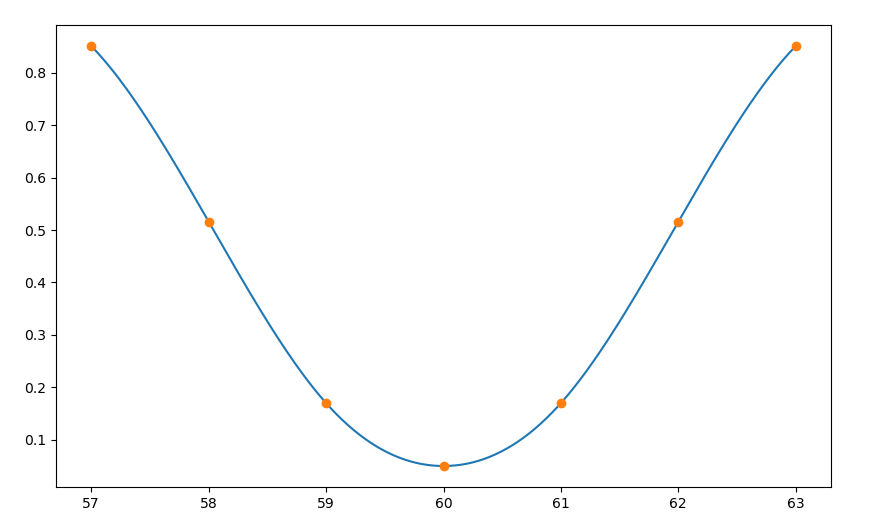
\includegraphics[width=0.7\textwidth]{6.4.4}
        \end{figure} \newpage
        %%%%%%%%%%%%%%%%%%%%%%%%%%%%%%%%%%%%%%%%%%%%%%%%%%%%%%%%%%%%%%%%%%%%%%%%%%%%%%%%%%%%%%%%%%%%%%%%%%%%         
        %%%%%%%%%%%%%%%%%%%%%%%%%%%%%%%%%%%%%%%%%%%%%%%%%%%%%%%%%%%%%%%%%%%%%%%%%%%%%%%%%%%%%%%%%%%%%%%%%%%%         
        %%%%%%%%%%%%%%%%%%%%%%%%%%%%%%%%%%%%%%%%%%%%%%%%%%%%%%%%%%%%%%%%%%%%%%%%%%%%%%%%%%%%%%%%%%%%%%%%%%%%         
        %%%%%%%%%%%%%%%%%%%%%%%%%%%%%%%%%%%%%%%%%%%%%%%%%%%%%%%%%%%%%%%%%%%%%%%%%%%%%%%%%%%%%%%%%%%%%%%%%%%%         
        %%%%%%%%%%%%%%%%%%%%%%%%%%%%%%%%%%%%%%%%%%%%%%%%%%%%%%%%%%%%%%%%%%%%%%%%%%%%%%%%%%%%%%%%%%%%%%%%%%%%    
    \item[]
        \textbf{Question 6.4.7} \\
        If $H_0:\mu=200$ is to be tested against $H_1:\mu < 200$ at the $\alpha = 0.10$ level of significance based
        on a random sample of size $n$ from a normal distribution where $\sigma = 15.0$, what is the smallest value
        for $n$ that will make the power equal to at least 0.75 when $\mu = 197$? \\
        \textbf{Solution} \\
        From \text{6.4}, the smallest sample size so that the power of a test to be at least 0.75 can be calculated as follows
        \begin{align*}
            P(\text{Reject}\;H_0\;|\;H_1\;\text{is true})                                     & \geq 0.75               \\
            P(\bar{y} < 200 + z_{\alpha = 0.10} \times \frac{\sigma}{\sqrt{n}}\;|\;\mu = 197) & \geq 0.75               \\
            P(\bar{y} < 200 - 1.28\times \frac{15}{\sqrt{n}}\;|\;\mu = 197)                   & \geq 0.75               \\
            P(\frac{\bar{y} - 197}{15 / \sqrt{n}} < \frac{3 - 19.2/\sqrt{n}}{15 / \sqrt{n}})  & \geq 0.75               \\
            P(z < \frac{3 - 19.2/\sqrt{n}}{15 / \sqrt{n}})                                    & \geq 0.75               \\
            \frac{3 - 19.2/\sqrt{n}}{15 / \sqrt{n}}                                           & \geq 0.675              \\
            3 - 19.2/\sqrt{n}                                                                 & \geq 10.125/\sqrt{n}    \\
            3                                                                                 & \geq 29.325/\sqrt{n}    \\
            \boldsymbol{n}                                                                    & \boldsymbol{\geq 95.55}
        \end{align*}
        Thus, the smallest value for $n$ that will make the power equal to at least 0.75 when $\mu = 197$ is $\boldsymbol{96}$.
        %%%%%%%%%%%%%%%%%%%%%%%%%%%%%%%%%%%%%%%%%%%%%%%%%%%%%%%%%%%%%%%%%%%%%%%%%%%%%%%%%%%%%%%%%%%%%%%%%%%%         
        %%%%%%%%%%%%%%%%%%%%%%%%%%%%%%%%%%%%%%%%%%%%%%%%%%%%%%%%%%%%%%%%%%%%%%%%%%%%%%%%%%%%%%%%%%%%%%%%%%%%         
        %%%%%%%%%%%%%%%%%%%%%%%%%%%%%%%%%%%%%%%%%%%%%%%%%%%%%%%%%%%%%%%%%%%%%%%%%%%%%%%%%%%%%%%%%%%%%%%%%%%%         
        %%%%%%%%%%%%%%%%%%%%%%%%%%%%%%%%%%%%%%%%%%%%%%%%%%%%%%%%%%%%%%%%%%%%%%%%%%%%%%%%%%%%%%%%%%%%%%%%%%%%         
        %%%%%%%%%%%%%%%%%%%%%%%%%%%%%%%%%%%%%%%%%%%%%%%%%%%%%%%%%%%%%%%%%%%%%%%%%%%%%%%%%%%%%%%%%%%%%%%%%%%%    
    \item[]
        \textbf{Question 6.4.9} \\
        If $H_0:\mu=30$ is tested again $H_1:\mu > 30$ using $n=16$ observations (normally distributed)
        and if $1 - \beta = 0.85$ when $\mu = 34$, what does $\alpha$ equal? Assume $\sigma = 9$. \\
        \textbf{Solution} \\
        From \textbf{6.4}, we know that $1 - \beta = P(\text{Reject}\;H_0\;|\;H_1\;\text{is true}) = 0.85$,
        thus, we can calculate $\bar{y}$ as follows
        \begin{align*}
            1 - \beta                                    & = P(\text{Reject}\;H_0\;|\;H_1\;\text{is true}) \\
            P(\bar{Y} > \bar{y} | \mu = 34)              & = 0.85                                          \\
            P(Z > \frac{\bar{y} - 34}{\sigma /\sqrt{n}}) & = 0.85                                          \\
            \frac{\bar{y} - 34}{\sigma / \sqrt{n}}       & \approx -1.035                                  \\
            \frac{\bar{y} - 34}{9 / \sqrt{16}}           & \approx -1.035                                  \\
            \bar{y}                                      & \approx 31.67
        \end{align*}
        From \textbf{6.2.1}, the test at the $\alpha$ level of significance can be calculated as follows
        \begin{align*}
            \alpha              & = P(\text{Reject}\;H_0\;|\;H_0\;\text{is true}) \\
            \alpha              & = P(\bar{y} > 31.67\;|\;\mu = 30)               \\
            \alpha              & = P(z > \frac{31.67 - 30}{9 / \sqrt{16}})       \\
            \alpha              & \approx P(z > 0.74)                             \\
            \boldsymbol{\alpha} & \boldsymbol{= 0.23}
        \end{align*}
        %%%%%%%%%%%%%%%%%%%%%%%%%%%%%%%%%%%%%%%%%%%%%%%%%%%%%%%%%%%%%%%%%%%%%%%%%%%%%%%%%%%%%%%%%%%%%%%%%%%%         
        %%%%%%%%%%%%%%%%%%%%%%%%%%%%%%%%%%%%%%%%%%%%%%%%%%%%%%%%%%%%%%%%%%%%%%%%%%%%%%%%%%%%%%%%%%%%%%%%%%%%         
        %%%%%%%%%%%%%%%%%%%%%%%%%%%%%%%%%%%%%%%%%%%%%%%%%%%%%%%%%%%%%%%%%%%%%%%%%%%%%%%%%%%%%%%%%%%%%%%%%%%%         
        %%%%%%%%%%%%%%%%%%%%%%%%%%%%%%%%%%%%%%%%%%%%%%%%%%%%%%%%%%%%%%%%%%%%%%%%%%%%%%%%%%%%%%%%%%%%%%%%%%%%         
        %%%%%%%%%%%%%%%%%%%%%%%%%%%%%%%%%%%%%%%%%%%%%%%%%%%%%%%%%%%%%%%%%%%%%%%%%%%%%%%%%%%%%%%%%%%%%%%%%%%%    
    \item[]
        \textbf{Question 7.3.2} \\
        Find the moment-generating function for a chi square random variable and use it to show that
        $E(\chi^2_n) = n$ and $V(\chi^2_n) = 2n$. \\
        \textbf{Solution} \\
        From \textbf{Theorem 7.3.1}, the moment-generating function for a chi square random variable is
        \begin{align*}
            M(t) & = E(e^{tX})                                                                            \\
                 & = \int_{-\infty}^{\infty} e^{tx} \frac{1}{2^{n/2} \Gamma(n/2)} x^{n/2 - 1} e^{-x/2} dx \\
                 & = \frac{1}{2^{n/2} \Gamma(n/2)} \int_{-\infty}^{\infty} x^{n/2 - 1} e^{-(1/2 - t)x} dx \\
        \end{align*}
        Let $u = -(1/2 - t)x$,
        then $du = -(1/2 - t)dx$, thus
        \begin{align*}
            M(t)              & = \frac{1}{2^{n/2} \Gamma(n/2)} \int_{-\infty}^{\infty} x^{n/2 - 1} e^{-(1/2 - t)x} dx                                      \\
            M(t)              & = \frac{1}{2^{n/2} \Gamma(n/2)} \int_{-\infty}^{\infty} \frac{u^{n/2 - 1}}{-(1/2 - t)^{n/2 - 1}} e^{u}\frac{du}{-(1/2 - t)} \\
            M(t)              & = \frac{1}{2^{n/2} \Gamma(n/2)} \frac{1}{-(1/2 - t)^{n/2}} \int_{-\infty}^{\infty} u^{n/2 - 1} e^{u} du                     \\
            M(t)              & = \frac{1}{2^{n/2} \Gamma(n/2)} \frac{1}{(1/2 - t)^{n/2}} \Gamma(n/2)                                                       \\
            \boldsymbol{M(t)} & \boldsymbol{= \frac{1}{(1 - 2t)^{n/2}}}
        \end{align*}
        We use the results above to show that $E(\chi^2_n) = n$  as follows
        \begin{align*}
            E(\chi^2_n)              & = M'(0)                                 \\
            E(\chi^2_n)              & = \frac{d}{dt} \frac{1}{(1 - 2t)^{n/2}} \\
            E(\chi^2_n)              & = \frac{d}{dt} (1 - 2t)^{-n/2}          \\
            E(\chi^2_n)              & = -\frac{n}{2} (1 - 2t)^{-n/2 - 1} (-2) \\
            \boldsymbol{E(\chi^2_n)} & \boldsymbol{= n}
        \end{align*}
        We use the results above to show that $V(\chi^2_n) = 2n$  as follows
        \begin{align*}
            V(\chi^2_n)              & = M''(0) - (M'(0))^2                                 \\
            V(\chi^2_n)              & = \frac{d^2}{dt^2} (1 - 2t)^{-n/2} - n^2             \\
            V(\chi^2_n)              & = \frac{d}{dt} (-n/2) (1 - 2t)^{-n/2 - 1} (-2) - n^2 \\
            V(\chi^2_n)              & = -4(\frac{-n}{2} - 1)\frac{-n}{2} - n^2             \\
            V(\chi^2_n)              & = 4(\frac{n^2}{4} + \frac{n}{2}) - n^2               \\
            \boldsymbol{V(\chi^2_n)} & \boldsymbol{= 2n}
        \end{align*}
        %%%%%%%%%%%%%%%%%%%%%%%%%%%%%%%%%%%%%%%%%%%%%%%%%%%%%%%%%%%%%%%%%%%%%%%%%%%%%%%%%%%%%%%%%%%%%%%%%%%%         
        %%%%%%%%%%%%%%%%%%%%%%%%%%%%%%%%%%%%%%%%%%%%%%%%%%%%%%%%%%%%%%%%%%%%%%%%%%%%%%%%%%%%%%%%%%%%%%%%%%%%         
        %%%%%%%%%%%%%%%%%%%%%%%%%%%%%%%%%%%%%%%%%%%%%%%%%%%%%%%%%%%%%%%%%%%%%%%%%%%%%%%%%%%%%%%%%%%%%%%%%%%%         
        %%%%%%%%%%%%%%%%%%%%%%%%%%%%%%%%%%%%%%%%%%%%%%%%%%%%%%%%%%%%%%%%%%%%%%%%%%%%%%%%%%%%%%%%%%%%%%%%%%%%         
        %%%%%%%%%%%%%%%%%%%%%%%%%%%%%%%%%%%%%%%%%%%%%%%%%%%%%%%%%%%%%%%%%%%%%%%%%%%%%%%%%%%%%%%%%%%%%%%%%%%%    
    \item[]
        \textbf{Question 7.4.5} \\
        Suppose a random sample of size $n=11$ is drawn from a normal distribution with $\mu = 15.0$. For what value of $k$
        is the following true?
        \begin{align*}
            P\big( \big| \frac{\bar{Y} - 15.0}{S/\sqrt{11}} \big| \geq k \big) = 0.05
        \end{align*}
        \textbf{Solution} \\
        Applying \textbf{7.4.1}, we construct a confidence interval for $\mu$ and solve for $k$ as follows
        \begin{align*}
            P\big(-t_{\alpha/2, n-1} \leq \frac{\bar{Y} - \mu}{S/\sqrt{n}} \leq t_{\alpha/2, n-1} \big) & = 1 - \alpha         \\
            P\big(-t_{0.025, 10} \leq \frac{\bar{Y} - 15.0}{S/\sqrt{11}} \leq t_{0.025, 10} \big)       & = 0.95               \\
            P\big(-2.228 \leq \frac{\bar{Y} - 15.0}{S/\sqrt{11}} \leq 2.228 \big)                       & = 0.95               \\
            P\big(\big| \frac{\bar{Y} - 15.0}{S/\sqrt{11}} \big| \geq 2.228 \big)                       & = 0.05               \\
            \boldsymbol{k}                                                                              & \boldsymbol{= 2.228}
        \end{align*}
        %%%%%%%%%%%%%%%%%%%%%%%%%%%%%%%%%%%%%%%%%%%%%%%%%%%%%%%%%%%%%%%%%%%%%%%%%%%%%%%%%%%%%%%%%%%%%%%%%%%%         
        %%%%%%%%%%%%%%%%%%%%%%%%%%%%%%%%%%%%%%%%%%%%%%%%%%%%%%%%%%%%%%%%%%%%%%%%%%%%%%%%%%%%%%%%%%%%%%%%%%%%         
        %%%%%%%%%%%%%%%%%%%%%%%%%%%%%%%%%%%%%%%%%%%%%%%%%%%%%%%%%%%%%%%%%%%%%%%%%%%%%%%%%%%%%%%%%%%%%%%%%%%%         
        %%%%%%%%%%%%%%%%%%%%%%%%%%%%%%%%%%%%%%%%%%%%%%%%%%%%%%%%%%%%%%%%%%%%%%%%%%%%%%%%%%%%%%%%%%%%%%%%%%%%         
        %%%%%%%%%%%%%%%%%%%%%%%%%%%%%%%%%%%%%%%%%%%%%%%%%%%%%%%%%%%%%%%%%%%%%%%%%%%%%%%%%%%%%%%%%%%%%%%%%%%%    
    \item[]
        \textbf{Question 7.4.9} \\

        \textbf{Solution} \\
        \begin{itemize}
            \item[(a)] First, we calculate $\bar{y}$ as follows
                \begin{align*}
                    \bar{y} & = \frac{1}{12}(40 + 34 + 23 + 40 + 31 + 33 + 49 + 33 + 34 + 43 + 26 + 39) \\
                            & = 35.41
                \end{align*}
                Applying \textbf{5.4.1}, we calculate samlpe standard deviation $S$ as follows
                \begin{align*}
                    S & = \sqrt{\frac{1}{n-1} \sum_{i=1}^{n} (y_i - \bar{y})^2} \\
                      & = \sqrt{\frac{1}{12-1} \sum_{i=1}^{12} (y_i - 35.41)^2} \\
                      & = 7.23
                \end{align*}
                Applying \textbf{7.4.1}, we construct a $95\%$ confidence interval as follows
                \begin{align*}
                    P\big(-t_{\alpha/2, n-1} \leq \frac{\bar{Y} - \mu}{S/\sqrt{n}} \leq t_{\alpha/2, n-1} \big) & = 1 - \alpha \\
                    P\big(-t_{0.025, 11} \leq \frac{\bar{Y} - 35.41}{7.23/\sqrt{12}} \leq t_{0.025, 11} \big)   & = 0.95       \\
                    P\big(-2.201 \leq \frac{\bar{Y} - 35.41}{7.23/\sqrt{12}} \leq 2.201 \big)                   & = 0.95       \\
                    P\big(\big| \frac{\bar{Y} - 35.41}{7.23/\sqrt{12}} \big| \geq 2.201 \big)                   & = 0.05       \\
                    \big| \frac{\bar{Y} - 35.41}{7.23/\sqrt{12}} \big|                                          & \geq 2.201   \\
                    \boldsymbol{30.81 \leq \bar{Y} \leq 40}
                \end{align*}
                Thus, for the $95\%$ confidence interval above, scientiests do their best job between 30.81 to 40 years old.
                \item[(b)]The graph of discovery by age over the year of discovery is as follows
                \begin{figure}[h]
                    \centering
                    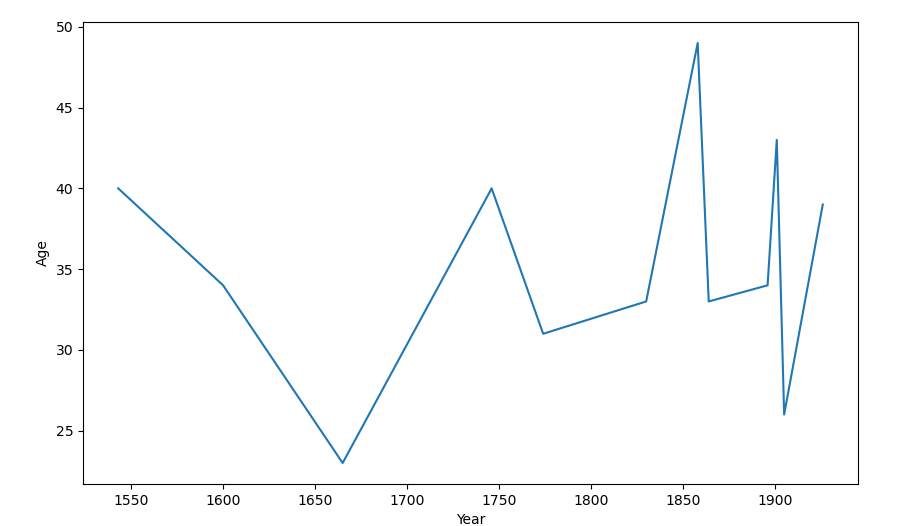
\includegraphics[width=0.7\textwidth]{7.4.2}
                \end{figure} \\
                From the graph above, the variability in the $y_i$'s appears to be random with respect to time.
        \end{itemize}
        %%%%%%%%%%%%%%%%%%%%%%%%%%%%%%%%%%%%%%%%%%%%%%%%%%%%%%%%%%%%%%%%%%%%%%%%%%%%%%%%%%%%%%%%%%%%%%%%%%%%         
        %%%%%%%%%%%%%%%%%%%%%%%%%%%%%%%%%%%%%%%%%%%%%%%%%%%%%%%%%%%%%%%%%%%%%%%%%%%%%%%%%%%%%%%%%%%%%%%%%%%%         
        %%%%%%%%%%%%%%%%%%%%%%%%%%%%%%%%%%%%%%%%%%%%%%%%%%%%%%%%%%%%%%%%%%%%%%%%%%%%%%%%%%%%%%%%%%%%%%%%%%%%         
        %%%%%%%%%%%%%%%%%%%%%%%%%%%%%%%%%%%%%%%%%%%%%%%%%%%%%%%%%%%%%%%%%%%%%%%%%%%%%%%%%%%%%%%%%%%%%%%%%%%%         
        %%%%%%%%%%%%%%%%%%%%%%%%%%%%%%%%%%%%%%%%%%%%%%%%%%%%%%%%%%%%%%%%%%%%%%%%%%%%%%%%%%%%%%%%%%%%%%%%%%%%    
    \item[]
        \textbf{Question 7.4.19} \\

        \textbf{Solution} \\
        First, we calculate $\bar{y}$ as follows
        \begin{align*}
            \bar{y} & = \frac{1}{15}(35 + 37 + 33 + 34 + 38 + 40 + 35 + 36 + 38 + 33 + 28 + 34 + 47 + 42 + 46) \\
                    & = 37.067
        \end{align*}
        Applying \textbf{5.4.1}, we calculate samlpe standard deviation $S$ as follows
        \begin{align*}
            S & = \sqrt{\frac{1}{n-1} \sum_{i=1}^{n} (y_i - \bar{y})^2}  \\
              & = \sqrt{\frac{1}{15-1} \sum_{i=1}^{15} (y_i - 37.067)^2} \\
              & = 5.049
        \end{align*}
        We can construct hypothesis as follows
        \begin{align*}
            H_0\!:\mu       & = 40                    \\
            H_1\!:\mu       & < 40                    \\
            n               & = 15                    \\
            \bar{y}         & = 37.067                \\
            S               & = 5.049                 \\
            \alpha          & = 0.05                  \\
            t_{\alpha, n-1} & = t_{0.05, 14} = 1.7613 \\
        \end{align*}
        From \textbf{Theorem 7.4.2}, we can test the hypothesis above as follows
        \begin{align*}
            \text{Reject}\;H_0\;\text{if}\;t & < -t_{\alpha, n-1}                                                                     \\
            \text{where}\;t                  & = \frac{\bar{y} - \mu_0}{S / \sqrt{n}} = \frac{37.067 - 40}{5.049 / \sqrt{15}} = -2.25 \\
            t                                & < -t_{\alpha, n-1}                                                                     \\
        \end{align*}
        Thus, we \textbf{reject} $\boldsymbol{H_0}$.
        %%%%%%%%%%%%%%%%%%%%%%%%%%%%%%%%%%%%%%%%%%%%%%%%%%%%%%%%%%%%%%%%%%%%%%%%%%%%%%%%%%%%%%%%%%%%%%%%%%%%         
        %%%%%%%%%%%%%%%%%%%%%%%%%%%%%%%%%%%%%%%%%%%%%%%%%%%%%%%%%%%%%%%%%%%%%%%%%%%%%%%%%%%%%%%%%%%%%%%%%%%%         
        %%%%%%%%%%%%%%%%%%%%%%%%%%%%%%%%%%%%%%%%%%%%%%%%%%%%%%%%%%%%%%%%%%%%%%%%%%%%%%%%%%%%%%%%%%%%%%%%%%%%         
        %%%%%%%%%%%%%%%%%%%%%%%%%%%%%%%%%%%%%%%%%%%%%%%%%%%%%%%%%%%%%%%%%%%%%%%%%%%%%%%%%%%%%%%%%%%%%%%%%%%%         
        %%%%%%%%%%%%%%%%%%%%%%%%%%%%%%%%%%%%%%%%%%%%%%%%%%%%%%%%%%%%%%%%%%%%%%%%%%%%%%%%%%%%%%%%%%%%%%%%%%%%    
    \item[]
        \textbf{Question 7.5.13} \\
        If a $90\%$ confidence interval for $\sigma^2$ is reported to be (51.47, 261.90),
        what is the value of the sample standard deviation? \\
        \textbf{Solution} \\
        From \textbf{Theorem 7.5.1}, we know that
        \begin{align*}
            (51.47, 261.90)                             & = \Big( \frac{(n-1)S^2}{\chi^2_{\alpha/2, n-1}}, \frac{(n-1)S^2}{\chi^2_{1-\alpha/2, n-1}} \Big) \\
            (51.47, 261.90)                             & = \Big( \frac{(n-1)S^2}{\chi^2_{0.05, n-1}}, \frac{(n-1)S^2}{\chi^2_{0.95, n-1}} \Big)           \\
            \frac{\chi^2_{0.95,n-1}}{\chi^2_{0.05,n-1}} & = \frac{261.90}{51.47}                                                                           \\
            \frac{\chi^2_{0.95,n-1}}{\chi^2_{0.05,n-1}} & = 5.088
        \end{align*}
        From \textbf{Table A3}, $n - 1 = 9$ with $\frac{16.919}{3.325} = 5.088$. \\
        Thus, sample standard deviation $S$ can be calculated as follows
        \begin{align*}
            \frac{(n-1)S^2}{\chi^2_{0.95, n-1}} & = 51.47                         \\
            S^2                                 & = \frac{51.47 \times 16.919}{9} \\
            S^2                                 & = 96.76                         \\
            \boldsymbol{S}                      & \boldsymbol{= 9.84}
        \end{align*}
        %%%%%%%%%%%%%%%%%%%%%%%%%%%%%%%%%%%%%%%%%%%%%%%%%%%%%%%%%%%%%%%%%%%%%%%%%%%%%%%%%%%%%%%%%%%%%%%%%%%%         
        %%%%%%%%%%%%%%%%%%%%%%%%%%%%%%%%%%%%%%%%%%%%%%%%%%%%%%%%%%%%%%%%%%%%%%%%%%%%%%%%%%%%%%%%%%%%%%%%%%%%         
        %%%%%%%%%%%%%%%%%%%%%%%%%%%%%%%%%%%%%%%%%%%%%%%%%%%%%%%%%%%%%%%%%%%%%%%%%%%%%%%%%%%%%%%%%%%%%%%%%%%%         
        %%%%%%%%%%%%%%%%%%%%%%%%%%%%%%%%%%%%%%%%%%%%%%%%%%%%%%%%%%%%%%%%%%%%%%%%%%%%%%%%%%%%%%%%%%%%%%%%%%%%         
        %%%%%%%%%%%%%%%%%%%%%%%%%%%%%%%%%%%%%%%%%%%%%%%%%%%%%%%%%%%%%%%%%%%%%%%%%%%%%%%%%%%%%%%%%%%%%%%%%%%%    
    \item[]
        \textbf{Question 7.5.16} \\
        Standard deviation: $\sigma = 1.0$ \\
        Hypothesis: $H_0\!:\sigma^2 = 1$ versus $H_1\!:\sigma^2 > 1$ \\
        Level of significance: $\alpha = 0.05$ \\
        $\sum_{i=1}^{30}y_1 = 758.2$ \\
        $\sum_{i=1}^{30}y_1^2 = 19195.7938$ \\
        \textbf{Solution} \\
        Applying \textbf{7.5}, we can calculate the sample variance $S^2$ as follows
        \begin{align*}
            S^2 & = \frac{30 \times 19195.7938 - 758.2^2}{30(30-1)} \\
                & = 0.425
        \end{align*}
        From \textbf{Theorem 7.5.2 (b)}, the critical value for the chi square ratio is
        \begin{align*}
            \chi^2_{1-\alpha, n-1} = \chi^2_{0.95, 29} = 42.557
        \end{align*}
        We can calculate the test statistic as follows
        \begin{align*}
            \chi^2 & = \frac{(n-1)S^2}{\sigma^2}          \\
            \chi^2 & = \frac{29 \times 0.425}{1}          \\
            \chi^2 & = 12.325                             \\
            \chi^2 & \leq \chi^2_{1-\alpha, n-1} = 42.557
        \end{align*}
        Thus, we \textbf{accept} $\boldsymbol{H_0}$
        %%%%%%%%%%%%%%%%%%%%%%%%%%%%%%%%%%%%%%%%%%%%%%%%%%%%%%%%%%%%%%%%%%%%%%%%%%%%%%%%%%%%%%%%%%%%%%%%%%%%    
        %%%%%%%%%%%%%%%%%%%%%%%%%%%%%%%%%%%%%%%%%%%%%%%%%%%%%%%%%%%%%%%%%%%%%%%%%%%%%%%%%%%%%%%%%%%%%%%%%%%%    
        %%%%%%%%%%%%%%%%%%%%%%%%%%%%%%%%%%%%%%%%%%%%%%%%%%%%%%%%%%%%%%%%%%%%%%%%%%%%%%%%%%%%%%%%%%%%%%%%%%%%    
        %%%%%%%%%%%%%%%%%%%%%%%%%%%%%%%%%%%%%%%%%%%%%%%%%%%%%%%%%%%%%%%%%%%%%%%%%%%%%%%%%%%%%%%%%%%%%%%%%%%%    
        %%%%%%%%%%%%%%%%%%%%%%%%%%%%%%%%%%%%%%%%%%%%%%%%%%%%%%%%%%%%%%%%%%%%%%%%%%%%%%%%%%%%%%%%%%%%%%%%%%%% 
\end{enumerate}
%%%%%%%%%%%%%%%%%%%%%%%%%%%%%%%%%%%%%%%%%%%%%%%%%%%%%%%%%%%%%%%%%%%%%%%%%%%%%%%%%%%%%%%%%%%%%%%%%%%%    
\end{document}